\documentclass[letterpaper, 12pt]{article}
\usepackage{graphics} 
\usepackage{amsmath} 
\usepackage{amssymb}
\usepackage{optidef}
\usepackage{derivative}
\usepackage[backend=biber]{biblatex}
\usepackage{hyperref}
\usepackage{cleveref}
\addbibresource{surface_planner.bib}

\title{Improving RRT* for a UAV with Dynamic Constraints in 3 Dimensions Using an Optimal Embedded Surface}
\author{Mike L. Sutherland, David A. Copp}

\begin{document}

\maketitle

\section{Introduction}
Unmanned Aerial Vehcles (UAVs) are increasingly used in many applications. Much attention has been devoted to Path Planning for UAVs, especially those with difficult dynamic constraints, such as fixed-wing aircraft. One of the significant tradeoffs in path planning is that of planning time, dimensionality, and complexity. Computing safe and optimal paths for UAVs with dynamic constraints can require significant computational complexity, especially if the configuration space has more then two dimensions.

We can clearly see this tradeoff at play in the family of algorithms based on the Rapidly-Exploring Random Tree (RRT) \cite{lavalle2006}. The Rapidly-Exploring Random Tree is frequently used for motion planning in high-dimensional spaces, because of its ability to compute paths that are approximately optimal. In fact, as more samples are drawn from the configuration space, the RRT path aproaches an optimal path. Because drawing each sample takes some finite time, plans generated by RRT algorithms are improved if the samples are drawn quicker. These qualities make RRT-like algorithms like a Monte Carlo method for a specific class of non-convex problem: the planning-with-constraints problem.

In thinking about the RRT planner as a non-convex optimization, we ask: can we reduce the size of the configuration space in an optimal way to improve planning times? 
Our strategy is to first reduce the 3-dimensional configuration space of a fixed-wing UAV to a 2-dimensional configuration space, by solving a convex problem. This 


\section{Definitions and Assumptions}
We assume a plan is computed over a 3-dimensional configuration space in $\mathbb{R}^3$. The first two dimensions of the configuration space are represented by a discrete grid, $\bar{X}$, which is a regular grid with each cell having length and width $d$. So, the first two dimensions of the configuration space are fixed in place as grid lattice points. The last dimension of the c-space in the $z$-direction is a real number which corresponds to the altitude of the grid point.

Therefore, the complete configuration space is given as an approximate surface, with each discrete grid point in $X$ corresponding to some real altitude $z$ -- forming the complete configuration space $\mathcal{X}$. We denote a point belonging to $X$ as $x$ and a point belonging to $\mathcal{X}$ as $\bar{x}$. We denote a point belonging to $\mathcal{X}_3$ as $z$.

To query the altitude of some off-grid point, it is assumed that a reasonable interpolation (nearest, linear, polynomial, etc.) can be performed to obtain an intermediate value of $z$.

\section{Algorithm}

At a high level, the steps of the algorithm are as follows:

\begin{itemize}
    \item Solve the convex problem
    \item Use the solution to the convex problem to inform the cost function of the RRT*
    \item Solve a 2-D RRT* problem with an altered cost function, $c(\bar{x})$, to obtain an optimal course over the sheet.\footnote{
My intuition says that the RRT cost function is isometric with the distance metric of the configuration space. This *seems* like a prerequisite for the RRT to approach optimality. And, that changes to the RRT cost function that preserve isometry between the two metrics are changes which preserve the property of the RRT which results in the RRT approaching optimality.

Like, that isometry between a cost functions $c$ and $c_\text{eu}$, is a *necessary* and *sufficient* condition for the RRT to find an optimal path through some type of euclidean C-space...

I've tried looking at papers that would explain this or proofs, but everything is so applied -- most use variants of the euclidean cost (if they change it at all), and they do not discuss the properties of the cost function that they use.

I think there is something very interesting and important about the cost function of the RRT that relates to its ability to solve this non-convex problem almost - optimally. Most papers are focused on getting the solution to converge faster on the euclidean metric, but hardly any are looking at the properties of the cost function! EDIT: there is one that uses artificial potential fields; \cite{} I think it could be very exciting to explore that more formally. I think it's crucial for actually explaining how solving the first convex problem, then using that solution inside of the RRT cost, makes the RRT converge to a better solution -- one which is informed by the information obtained from the convex problem.}
\end{itemize}

Each $x \in X$ has some terrain below it, with some height $z_\text{obs}$. Our goal is to compute a real-valued plan elevation, $z$, for all $x \in X$, bearing in mind $z_\text{obs}$, our vehicle dynamics as they relate to the $z$-dimension, and any additional heuristics.

This convex problem can be written:

\begin{mini!}
    {J}{J = z}
    {\label{eq:Example1}}
    {}
    \addConstraint{ z }{ \geq z_\text{min} }
    \addConstraint{ z - z_\text{gap} }{ \geq z_\text{obs} }
    \addConstraint{ \pdv{z}{x} }{ \leq v_\text{max} }
    \addConstraint{ \frac{\partial ^2 z}{x^2} }{ \leq a_\text{max} } % 2nd partial derivative package does not work in mini! environment
\end{mini!}

Where $z$ is the vehicle height and $z_\text{obs}$ is the obstacle height. $v_\text{max}$ is the maximum climb rate of the vehicle, $a_\text{max}$ is the maximum vertical acceleration of the vehicle, and $z_\text{gap}$ is the minimum gap between the vehicle height and the height of an obstacle.

Solving the convex problem gives us an optimal cost for each point in the configuration space. We can think of this cost as an ``elevation.'' Indeed, in the UAV inspection task, we are trying to fly as low as possible. Then, computing a plan between $x_1$ and $x_2 \in X$ and projecting onto $\mathcal{X}$ will produce a valid plan which will direct the UAV to a safe and optimal height, even under the vehicle's vertical climb and acceleration constraints.


However, we can also improve our RRT by altering its cost function with an additional heuristic informed by this new elevation data. We use the RRT* algorithm, but replacing the standard euclidean cost function

\begin{equation}
c_\text{eu}(\bar{x}_1, \bar{x}_2) = |(x_2 - x_1)|
\end{equation}


With a new cost function. Let $l_{12}$ be a collection of points in $X$, each of which is some distance from a straight line from $x_1$ to $x_2$,

\begin{equation}
l_{12} = \{x \in X | \min(|x - l_{12}|) \leq u \},
\end{equation}

where $u \geq d$. Algorithms such as Bresenham's Straight Line algorithm can be used to compute such collections quickly. The z-values of these points (in $\mathcal{X}$-space) are their ``elevations'' on the sheet. Call this collection of z-values $\mathcal{Z^\text{line}}$. We then plan in $X$ using the cost function
\begin{equation}
c_\text{sheet}(x_1, x_2) = |x_2 - x_1| + \gamma_z \cdot |x_2 - x_1| \cdot \sum^k_i({\frac{z_i}{k}})
\end{equation}

\footnote{
Probably, we need to prove that this cost function forms a metric space $(\mathcal{X}, c)$: positivity, symmetry,  triangle inequality. I think I can use some clever properties of each term and the composition thereof to do this succinctly.}

Where $\gamma_z$ is a scaling factor, $|x_2-x_1|$ is the $\mathbb{R}^2$ distance between the points, and $z_i$ is the elevation of the $i$ th point in a collection of $k$ points formed by the line $l_{12}$. Note that when the scaling factor $\gamma_z=0$, $c_\text{sheet}$ reduces to $c_\text{eu}$. This factor represents a cost penalty on the elevation of each point between the points $x_1$ and $x_2$. 

\section{Results}
\begin{figure}
    \centering
    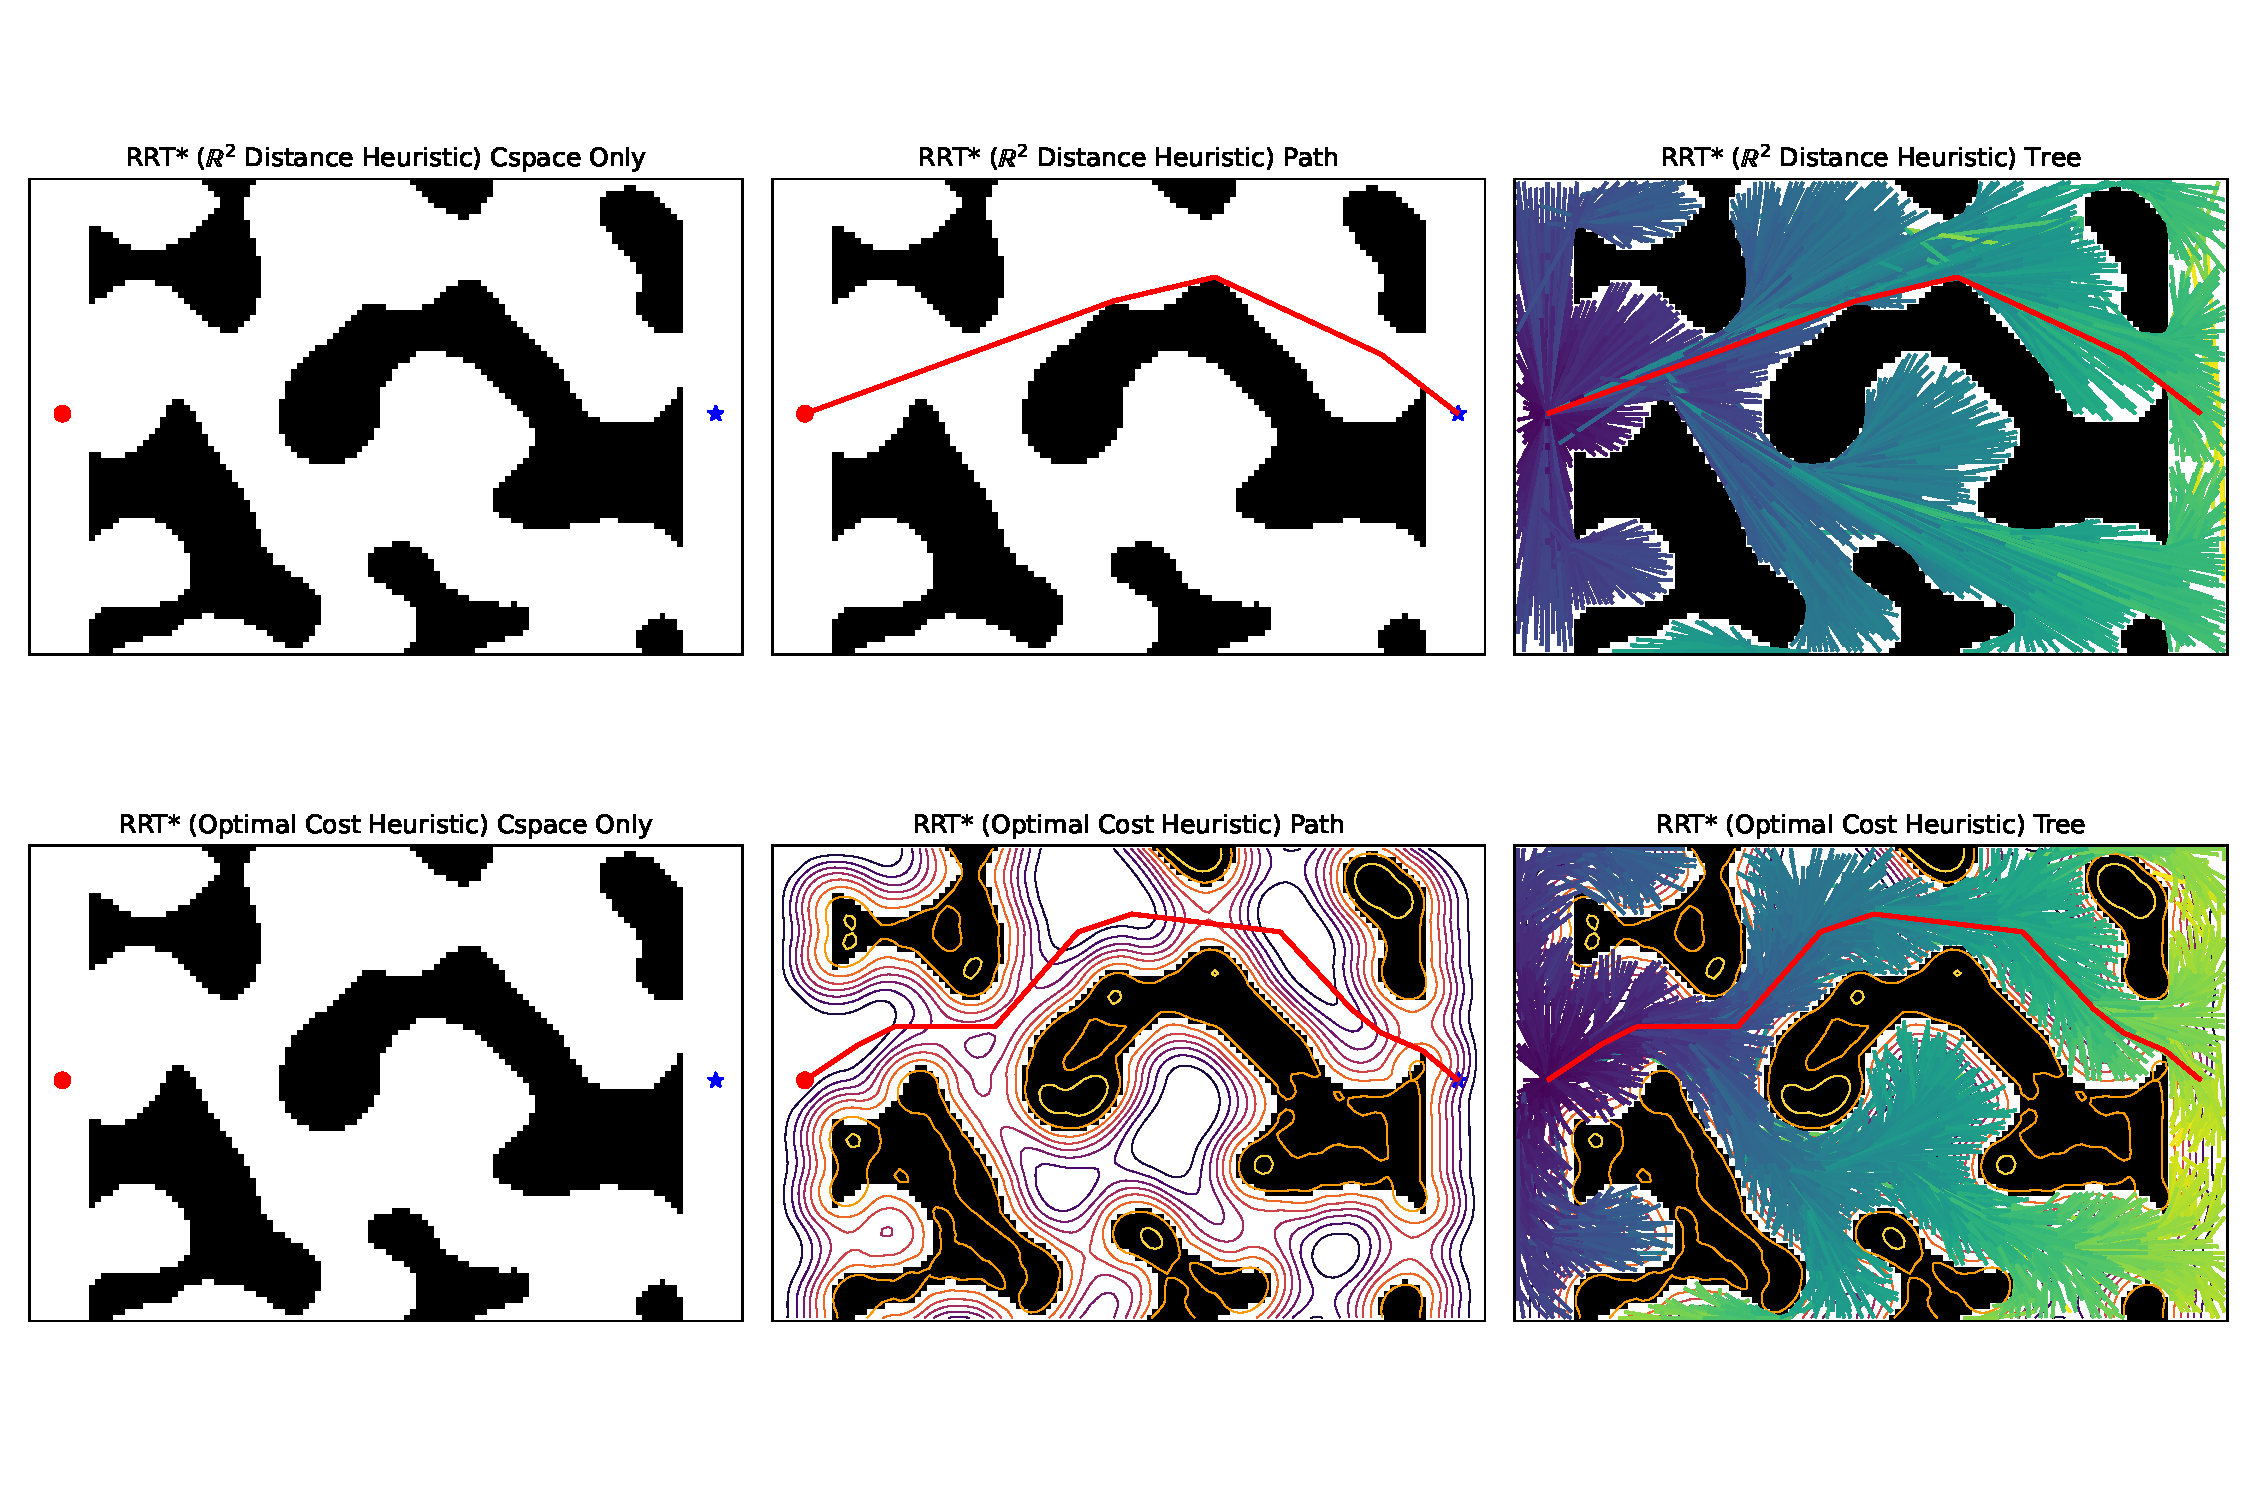
\includegraphics[width=0.9\linewidth]{./figures/rrt_surface_fig.pdf}
    \caption{A comparison between the RRT* algorithm (n=4000) run with the standard Euclidean cost function (top row) and a cost function with a penalty on the elevation of the point in the $z$-dimension (bottom row). The first column shows the configuration space, which is the same between both planners. The second column (in the second row) shows the contour lines of $z$-elevation of the computed surface, with the obstacles treated as elevated terrain. Finally, the tree and computed paths are shown. We see a more cautious path, in the bottom row, since $z$-elevation is punished in the RRT* cost function and the elevation is higher near obstacles.}
\end{figure}

\printbibliography

\end{document}
